\documentclass{article}
\usepackage{graphicx}
\usepackage{verbatim}
\usepackage[margin=1in]{geometry}
\usepackage{enumitem}
\usepackage{amsmath,amssymb}
\usepackage{bm}
\usepackage{stmaryrd}
\title{Understanding Reflux}
\author{B. Runnels and V. Agrawal}
\begin{document}
\maketitle
\setlength\parindent{0pt}
\def\flux{\operatorname{Flux}}
\def\Int{\operatorname{int}}


\section{Interpretation as integral of flux jump}
Let $\Omega\subset\mathbb{R}^n$ be the problem domain, and let $A:C^2(\Omega)\to C^0(\Omega)$ be a linear operator.
In the implementation of \texttt{amrex::MLNodeLaplacian}, $A$ has the form
\begin{align}
  A[\phi](\bm{x}) = \nabla\cdot\bm{\sigma}(\bm{x})\nabla\phi, 
\end{align}
where $\bm{\sigma}:\Omega\to\mathbb{R}^{n\times n}$ is a coefficient matrix\footnote{Appears to be implemented in \texttt{amrex} as a vector, corresponding to a diagonal matrix}.
The corresponding {\it flux} of the operator $\bm{f}_A:C^1(\Omega)\to C^0(\Omega,\mathbb{R}^n)$ is
\begin{align}
  \bm{f}_A[\phi](\bm{x}) = \bm{\sigma}(\bm{x})\nabla\phi
\end{align}
The pointwise residual is defined as 
\begin{align}
  r(\bm{x}) = b(\bm{x}) - A[\phi](\bm{x})
\end{align}
where $b:\Omega\to\mathbb{R}$ is the right hand side.
The {\it total residual} is the integral 
\begin{align}
  R = \int_\Omega r(\bm{x})\,d\bm{x}
\end{align}
Let $B\subset\Omega$ represent the {\it refined region} and $\Omega\setminus B$ the {\it coarse region}.
By nature of the discrete algorithm, we assume that $\nabla\phi$ is discontinuous over the boundary $\partial B$.
\begin{align}\label{eq:resorig}
  R = \int_\Omega b(\bm{x})\,d\bm{x} - \int_{B} A[\phi](\bm{x})\,d\bm{x} - \int_{\Omega\setminus B} A[\phi](\bm{x})\,d\bm{x}
\end{align}
Using the divergence theorem this reduces to
\begin{align}
  R = \int_\Omega b(\bm{x})\,d\bm{x} - \int_{\partial \Omega} \bm{n}\cdot\bm{f}_A[\phi](\bm{x})\,d\bm{x} - \int_{\partial B} \bm{n}\cdot\bm{f}^{B}_A[\phi](\bm{x})\,d\bm{x} + \int_{\partial B} \bm{n}\cdot\bm{f}^{\Omega\setminus B}_A[\phi](\bm{x})\,d\bm{x}
\end{align}
where $\bm{n}$ is the outward-facing normal for $B$.
The superscripts on $\bm{f}$ indicate where the flux is computed: $\bm{f}_A^{B}$ is evaluated on $B$, $\bm{f}_A^{\Omega\setminus B}$ on $\Omega\setminus B$.
This is alternatively expressed using jump-bracket notation,
\begin{align}
  R = 
  \int_\Omega b(\bm{x})\,d\bm{x} 
  - \int_{\partial \Omega} \bm{n}\cdot\bm{f}_A[\phi](\bm{x})\,d\bm{x}
  - \int_{\partial B} \bm{n}\cdot\Big\llbracket\bm{f}_A[\phi](\bm{x})\Big\rrbracket\,d\bm{x}.
\end{align}
An additional application of the divergence theorem to the second term yelds the result
\begin{align}\label{eq:rhscfreflux}
  R = 
  \underbrace{\int_\Omega b(\bm{x})\,d\bm{x} }_{\text{r.h.s.}}
  - \underbrace{\int_{\Int(\Omega\setminus B)} A[\phi](\bm{x})\,d\bm{x}}_{\text{coarse}}
  - \underbrace{\int_{\Int(B)} A[\phi](\bm{x})\,d\bm{x}}_{\text{fine}}
  - \underbrace{\int_{\partial B} \bm{n}\cdot\Big\llbracket\bm{f}_A[\phi](\bm{x})\Big\rrbracket\,d\bm{x}}_{\text{reflux}}.
\end{align}
We note that (\ref{eq:rhscfreflux}) is nearly identical to (\ref{eq:resorig}) except for the additional boundary integral. 
This is the result of the discretization and subsequent loss of continuity at the boundary.
\begin{enumerate}
\item In the continuous case, the jump term $\llbracket\bm{f}_A\rrbracket$ would be zero and would consequently vanish.
  Including it explicitly accounts for the reflux contribution at the coarse/fine boundary.
\item Terms 2 and 3 are now over the {\it interiors} of $\Omega\setminus B,B$.
  This is a trivial distinction in the continuous case, but is meaningful in the discrete case as it indicates that the boundary nodes are not included in the coarse and fine contributions.
\end{enumerate}


\section{Multi-level stencil}

Consider a multi-level stencil in which the solution on the coarse level is $pc$ and on the fine level is $pf$.
We wish to estimate the second derivative in the $x$ direction at coarse/fine boundary node $(i,j)$ using both coarse and fine nodes.
We assume that $pc(i,j) = pf(2i,2j)$.

\begin{center}
  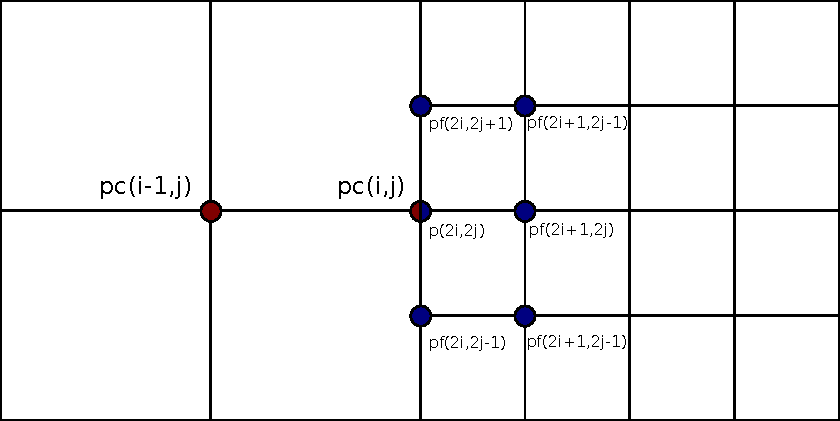
\includegraphics{stencil1}
\end{center}

We first compute finite difference first derivatives on the coarse and fine levels, denoting them as $dpc,dpf$, respectively.
The values ``live'' half way between the two stencil points, as shown below:

\begin{center}
  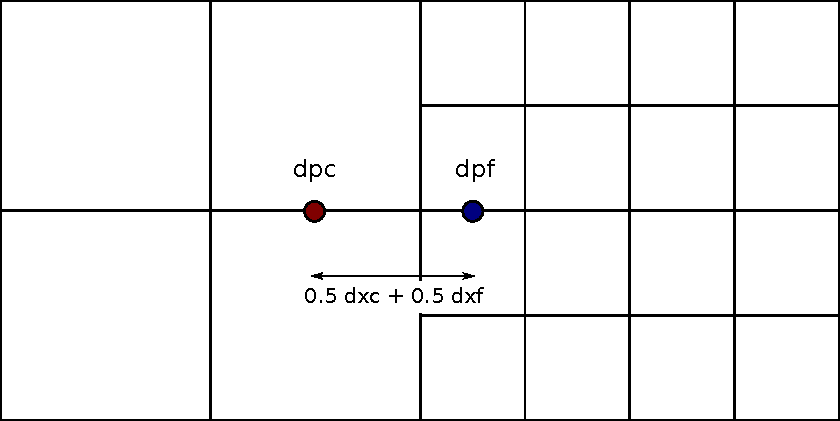
\includegraphics{stencil2}
\end{center}

The coarse derivative is just
\begin{align}
  pc = \frac{pc(i,j) - pc(i-1,j)}{dxc}.
\end{align}
The fine derivative is a weighted average:
\begin{align}
  pf = 
  \frac{1}{2}\frac{pf(2i+1,j) - pc(i,j)}{dxf}
  + \frac{1}{4}\frac{pf(2i+1,j+1) - pc(i,j+1)}{dxf}
  + \frac{1}{4}\frac{pf(2i+1,j-1) - pc(i,j-1)}{dxf}
\end{align}
Then the second derivative at $(i,j)$ is computed by finite difference between the two first derivatives
\begin{align}
  ddpc(i,j) = \frac{pf - fc}{(dxf/2) + (dxc/2)}
\end{align}
and lives at the coarse fine node
\begin{center}
  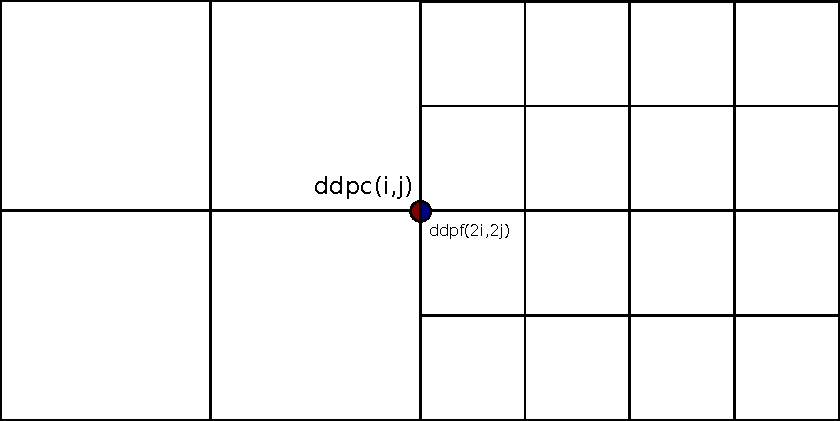
\includegraphics{stencil3}
\end{center}
The location of this node means that the derivative is a combination of central and backward differencing.



\end{document}


